%%%%%%%%%%%%%%%%%%%%%%%%%%%%%%%%%%%%%%%%%%%%%%%%%%%%%%%%%%%%
\section{The Agentic AI Trust Layer}
\label{sec:trust-layer}

In this section we describe an Agentic AI Trust Layer, which includes authenticated workflows and authenticated prompts and context as described in~\cite{rajagopalan2025prompts}. All nine frameworks map onto the trust layer using thin framework adapters. The trust layer comprises a control plane providing core services (identity, policy, logging, routing), manages integrations with enterprise infrastructure (IAM, PKI, storage, etc), a verification gateway (sidecar PEP) and client libraries that embed PEPs within agentic applications. Due to space we focus our discussion on key design elements instead of an exhaustive overview.

\begin{figure}[t]
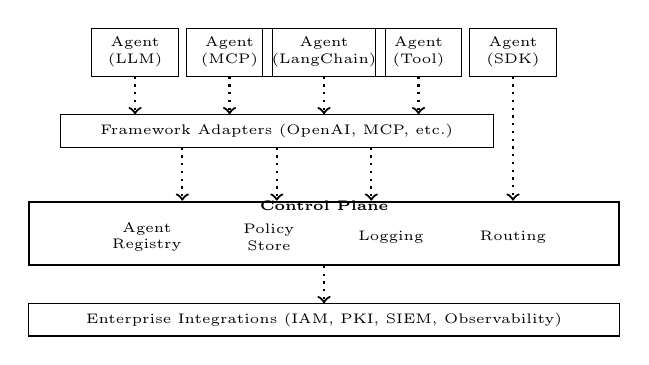
\begin{tikzpicture}[
  agent/.style={rectangle, draw, minimum width=1.1cm, minimum height=0.4cm, font=\tiny, align=center},
  integration/.style={rectangle, draw, minimum width=7.5cm, minimum height=0.4cm, font=\tiny, align=center},
  service/.style={rectangle, minimum width=1.65cm, minimum height=0.5cm, font=\tiny, align=center},
  adapter/.style={rectangle, draw, minimum width=5.5cm, minimum height=0.4cm, font=\tiny, align=center}
]

% Top layer: 5 Agents
\node[agent] (agent1) at (-2.4,0) {Agent\\(LLM)};
\node[agent] (agent2) at (-1.2,0) {Agent\\(MCP)};
\node[agent] (agent3) at (0,0) {Agent\\(LangChain)};
\node[agent] (agent4) at (1.2,0) {Agent\\(Tool)};
\node[agent] (agent5) at (2.4,0) {Agent\\(SDK)};

% Framework Adapters layer (narrower, slightly wider to accommodate 4 agents)
\node[adapter] (adapters) at (-0.6,-1) {Framework Adapters (OpenAI, MCP, etc.)};

% Control Plane box (full width, reduced height)
\node[draw, thick, rectangle, minimum width=7.5cm, minimum height=0.8cm] (controlplane-box) at (0,-2.3) {};

% Control Plane label (centered at top inside box, bold)
\node[font=\tiny\bfseries] at (0,-1.95) {Control Plane};

% Services inside control plane - single row, all same size
\node[service] (registry) at (-2.25,-2.35) {Agent\\Registry};
\node[service] (policy) at (-0.7,-2.35) {Policy\\Store};
\node[service] (logging) at (0.85,-2.35) {Logging};
\node[service] (routing) at (2.4,-2.35) {Routing};

% Bottom layer: Enterprise Integrations
\node[integration] (integrations) at (0,-3.4) {Enterprise Integrations (IAM, PKI, SIEM, Observability)};

% Arrows: First 4 agents to Framework Adapters (vertical)
\draw[->, thick, dotted] (agent1.south) -- (agent1.south |- adapters.north);
\draw[->, thick, dotted] (agent2.south) -- (agent2.south |- adapters.north);
\draw[->, thick, dotted] (agent3.south) -- (agent3.south |- adapters.north);
\draw[->, thick, dotted] (agent4.south) -- (agent4.south |- adapters.north);

% Arrows: 3 parallel vertical arrows from Framework Adapters to Control Plane
\draw[->, thick, dotted] ([xshift=-1.2cm]adapters.south) -- ([xshift=-1.2cm]adapters.south |- controlplane-box.north);
\draw[->, thick, dotted] (adapters.south) -- (adapters.south |- controlplane-box.north);
\draw[->, thick, dotted] ([xshift=1.2cm]adapters.south) -- ([xshift=1.2cm]adapters.south |- controlplane-box.north);

% Arrow: Direct SDK agent bypasses adapters to Control Plane (vertical)
\draw[->, thick, dotted] (agent5.south) -- (agent5.south |- controlplane-box.north);

% Control Plane connects to Enterprise Integrations (vertical)
\draw[->, thick, dotted] (controlplane-box.south) -- (integrations.north);

\end{tikzpicture}
\caption{Agentic AI Trust Layer.}
\label{fig:runtime-architecture}
\end{figure}

\subsection{Architecture}

Figure~\ref{fig:runtime-architecture} shows the trust layer architecture with agents interfacing with the control plane.

\textbf{Framework Adapters}. Each framework integrates through thin adapters that translate framework-native operations into authenticated workflows. Adapters implement the four-phase protocol—registration, invocation signing, verification, and attestation—while presenting the framework's native API. Integration is transparent; developers use standard framework APIs (MCP servers, OpenAI clients, LangChain agents) while cryptographic enforcement happens automatically.

\textbf{Control Plane Services}. The control plane provides four core services:
\begin{itemize}
\item \textit{Agent Registry}: Stores agent identifiers and public keys, and tool identifiers and public keys within agents, preserving cryptographic lineage. Enables instant credential revocation. PEPs retrieve public keys during signature verification.

\item \textit{Policy Store}: Tamper-proof policy store where PEPs retrieve and compose hierarchical policies (e.g., company, business unit, team) through intersection.

\item \textit{Routing}: Routes signed invocations between agents across network boundaries, enabling callees to access callers' public keys for verification.

\item \textit{Logging}: Records all security events with cryptographic lineage through tamper-evident hash chains. Integrates with enterprise SIEM platforms. Blocked operations generate structured logs indicating rejection reason (signature invalid, policy violation, missing attestation, verifier failure) with sufficient detail for debugging while avoiding policy leakage. Audit logs enable root-cause analysis and compliance reporting.
\end{itemize}

\textbf{Distributed Enforcement}. These services run in highly available configurations, integrating with enterprise infrastructure (IAM, PKI, SIEM, observability platforms). The control plane is multi-tenant—organizations deploy shared infrastructure while maintaining cryptographic isolation between tenants. The architecture realizes zero-trust distributed verification—each PEP independently verifies invocations using public keys from the registry and policies from the store. 
PEPs are embedded in-process by default (linked library) or deployed as sidecars, providing horizontal scalability. 
With embedded PEPs, no centralized bottleneck exists; verification happens locally at each boundary with sub-millisecond overhead. 
Administrators can instantly revoke credentials, update policies, or isolate agents through the control plane. Due to space constraints, full architectural details are out of scope; we refer interested readers to our technical report for complete implementation details.

\subsection{Design Decisions}

Realizing authenticated workflows and our trust layer in production exposed several practical challenges that needed an opinionated design—we discuss six of the most interesting design decisions addressing these challenges.

\textbf{Identity Bridging}. Enterprise identities need bridging across frameworks—each has its own authentication model (OAuth, API keys, SAML). Instead of solving this per-framework, we bridge at the protocol level. When users authenticate, the trust layer issues ephemeral keypairs bound to their sessions and propagates cryptographically-verified principals across all frameworks. Signed invocations carry user identity through delegation chains; each PEP independently verifies the originating principal from the Agent Registry. This centralizes IAM integration—frameworks don't individually integrate with corporate identity systems; the trust layer handles authentication once. When OAuth-authenticated Alice invokes API-key-authenticated Claude which calls MCP-authenticated tools, logs show "Alice via Claude accessed file" preserving audit trails. Protocol-level bridging provides a simpler programming model with consistent principal propagation, eliminating per-framework integration complexity.

\textbf{Session Management}. Many frameworks lack native session concepts (MCP, LangChain are stateless), yet cross-turn correlation is essential for security. Instead of modifying each framework to add sessions, we track at the protocol level using context identifiers and sequence numbers transparent to frameworks. The trust layer maintains authenticated context regardless of framework support—frameworks without sessions receive invisible protocol-level tracking; frameworks with sessions map directly. Multi-tenant architecture ensures cryptographically isolated contexts per session, preventing cross-session contamination. This enables unified audit trails across multi-framework workflows without requiring protocol modifications to individual frameworks.

\textbf{Verifiable Delegation}. Multi-hop delegation creates privilege escalation risks—compromised intermediate agents could claim broader permissions than granted. Instead of trust-based delegation, we enforce cryptographic scope narrowing. Signed delegation tokens contain delegator identity, delegate identity, scope constraints, and expiration. The trust layer enforces scope narrowing via intersection: delegated scope = what delegator grants $\cap$ what delegate possesses, extending MAPL's algebra (Section~\ref{sec:policy}). Compromised agents cannot claim broader permissions than granted; downstream services cryptographically verify delegation validity. This provides provable least privilege across heterogeneous frameworks.

\textbf{Forward Secrecy}. Long-lived API keys create operational and security risks—keys rarely rotate, and a single leak compromises all sessions. Instead of relying on operational key rotation policies, we use ephemeral keys by design. Each session receives unique ephemeral keypairs that expire automatically. Key rotation happens naturally via session lifecycle without infrastructure modifications, providing session-level forward secrecy. Compromising one session's key doesn't affect other sessions, limiting blast radius without operational overhead.

\textbf{Service Accounts at Scale}. Agentic systems spawn entities dynamically at runtime—orchestrators spawn agents, agents spawn tools, workflows create sub-workflows. Traditional IAM's manual provisioning doesn't scale to runtime dynamics. Instead of manual provisioning, we automatically provision cryptographic identities during registration (Section~\ref{sec:authenticated-workflows}) at tool-level granularity—assigning (tool\_id, keypair) and recording in the Agent Registry. No manual provisioning, no credential distribution, no IAM bottleneck. Each tool maintains independent cryptographic accountability, minimizing blast radius. This enables dynamic agent deployment at enterprise scale.

\textbf{Bidirectional Accountability}. Unidirectional authentication creates accountability gaps in agentic environments—callers cannot prove services performed operations correctly; services cannot prove callers requested operations. Instead of one-way signatures, we use dual signatures for mutual non-repudiation. Callers sign requests; services sign results. Each operation produces cryptographic proof from both parties, providing compliance-grade audit trails—services cannot repudiate actions; callers cannot repudiate requests. Combined with identity bridging and tamper-evident logging, this delivers complete accountability across heterogeneous authentication boundaries.
